This section specifies the software architecture requirements and the software
architecture design at the second level of granularity - the benchmark monitor
application. The monitor will be responsible for benchmarking a user application.

\section{Monitor}
\subsection{Architecture Requirements}
This section discusses the software architecture requirements around the
back end benchmark system infrastructure. The monitor will be responsible for
retrieving a job specification from the queue, building, compiling and
benchmarking a user application based on the job specification. A key concept
in the design of the monitor nodes was to ensure monitor nodes remain autonomous
to allow for the addition and removal of monitor nodes.
In particular the architecture requirements at the second level of
granularity is specified.

Figure \ref{fig:benchmarkInfrastructure} show the a high-level infrastructure
view of the Benchmark Monitor service.

\begin{figure}[H]
  \begin{center}
  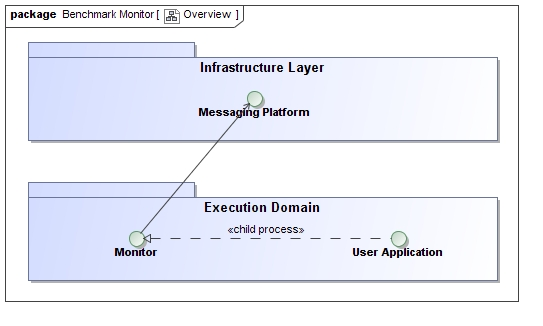
\includegraphics[scale=0.4]{../Diagrams and Charts/Overview/BenchmarkInfrastructure.jpg}
  \caption{A high-level overview of the software architecture for the Benchmark Service}
  \label{fig:benchmarkInfrastructure}
  \end{center}
\end{figure}


\subsubsection{Access and Integration Requirements}
\label{sec:accessIntegrationRequirementsManagementSystem}
\paragraph*{Access Channels}
No human access channels are present with the monitor application. A system
access channel however is present, allowing the monitor node to communicate with
the back end management system through the messaging platform. The messaging
platform provides a highly decoupled system, allowing nodes to come and go as
necessary. To assist the administrator to monitor the nodes, the management
platform implements a monitoring system where nodes can send heartbeat messages
to alert the management system of the individuals status. Message can indicate
if a node is online and waiting to retrieve jobs, if a host is going to start a
benchmark or if a node is shutting down.

\subsubsection{Quality Requirements}
No additional quality requirements are imposed on the system other than that
defined in section \label{sec:overallQualityRequirement}.

\subsection{Architecture Design}
\subsubsection{Architectural Responsibilities, Components and Realization}
The architectural responsibilities, components and concrete realization of these 
responsibilities are shown in 
Figure \ref{fig:databaseResponsibilityRealization}
\begin{figure}[H]
	\begin{center}
	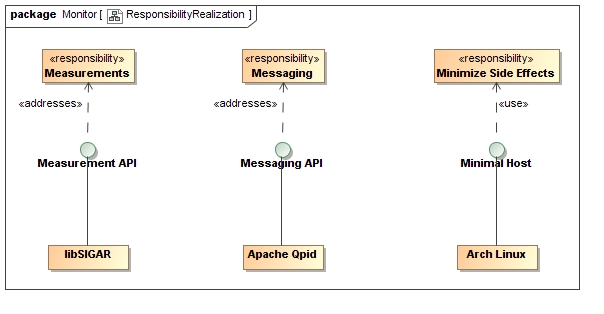
\includegraphics[scale=0.5]{../Diagrams and Charts/Monitor/ResponsibilityRealization.jpg}
	\caption{The components with which the architecture responsibilities within the monitor is realized}
	\label{fig:databaseResponsibilityRealization}
	\end{center}
\end{figure}

\subsubsection{Tactics}
As the monitor node must ensure accurate benchmarking, it is important to keep
the monitor node small and eliminate side effects as far as possible. Tactics
to  address the quality requirements include:
\begin{itemize}
	\item \textit{Accurate measurements} must be made when benchmarking the user
    applications. For this reason an existing library that is used by the greater
    academic community will be used to make the measurements.
	\item \textit{Minimizing side effects} will be done by setting up a minimal
    host operating system, as to minimize, threads running, interrupts and
    paging. To accomplish this, a minimal Linux host will be setup, will all but
    the bare components required to accomplish the task of benchmarking.
	\item \textit{Communicate synchronously} with the queue, to ensure no side
    effects is introduced. Communication with the queue will only occur when
    no benchmarking is being done on the host.
\end{itemize}

\subsubsection{Frameworks and Technologies}
\paragraph*{libSIGAR} As we require accurate measurements, it is very important
  to use a library that has been battle-tested in an academic environment. After
  extensive research, we noticed that the libSIGAR library is use in multiple
  research projects, is discussed in academic papers and seem to be the current
  library used to do benchmarking with.
\paragraph*{Apache Qpid and Proton} As C++ doesn't have native support for 
  communication with a message broker, we require a library that provides support
  for the AMQPv1 protocol. Apache Qpid together with Apache Proton, providers
  support to C++ to allow communication with an AMQP broker.
\paragraph*{YAML CPP} To assist the administrator of the benchmarking service
  in monitoring node, while keeping nodes autonomous and ephemeral, we will allow
  the operator of a benchmarking node to configure a YAML file with information
  related to the node which he/she is operating. This information will then be
  forwarded to the management system by way of the messaging platform, which
  will allow the administrator of the benchmarking system to monitor nodes.
